\chapter{Abbildungen}
\begin{sidewaysfigure}[ht]
	\centering
	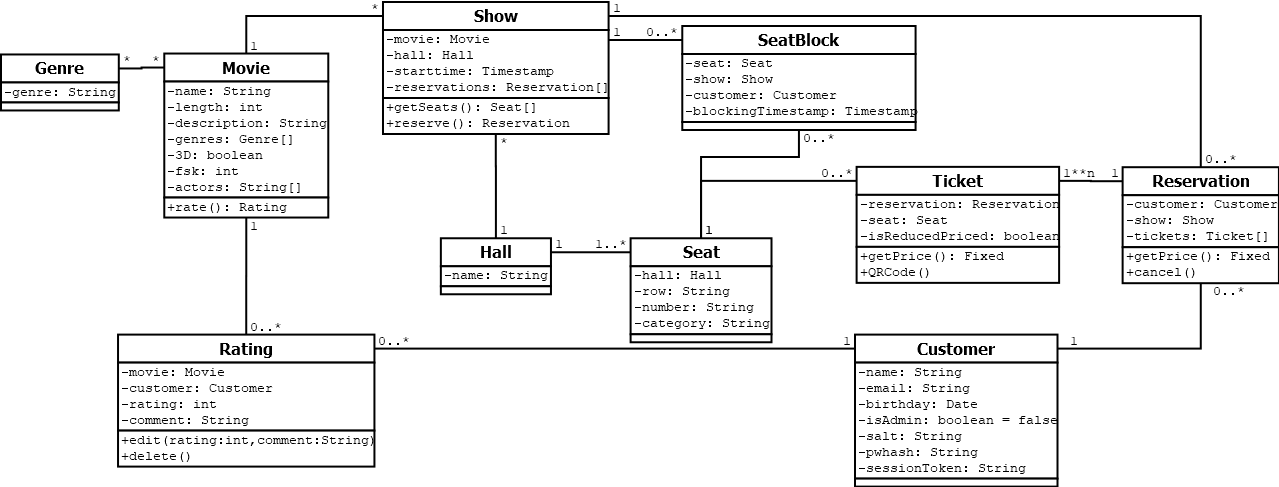
\includegraphics[keepaspectratio, width=\textwidth, height=\textheight]{img/klassendiagramm_v01}
	\captionsetup{format=hang}
	\caption{Erster Entwurf des Klassendiagramms}
	\small Quelle: eigene Darstellung mittels \url{http://dia-installer.de/index.html.de}
	\label{fig:anhang_klassendiagramm01}
\end{sidewaysfigure}

\begin{sidewaysfigure}[ht]
	\centering
	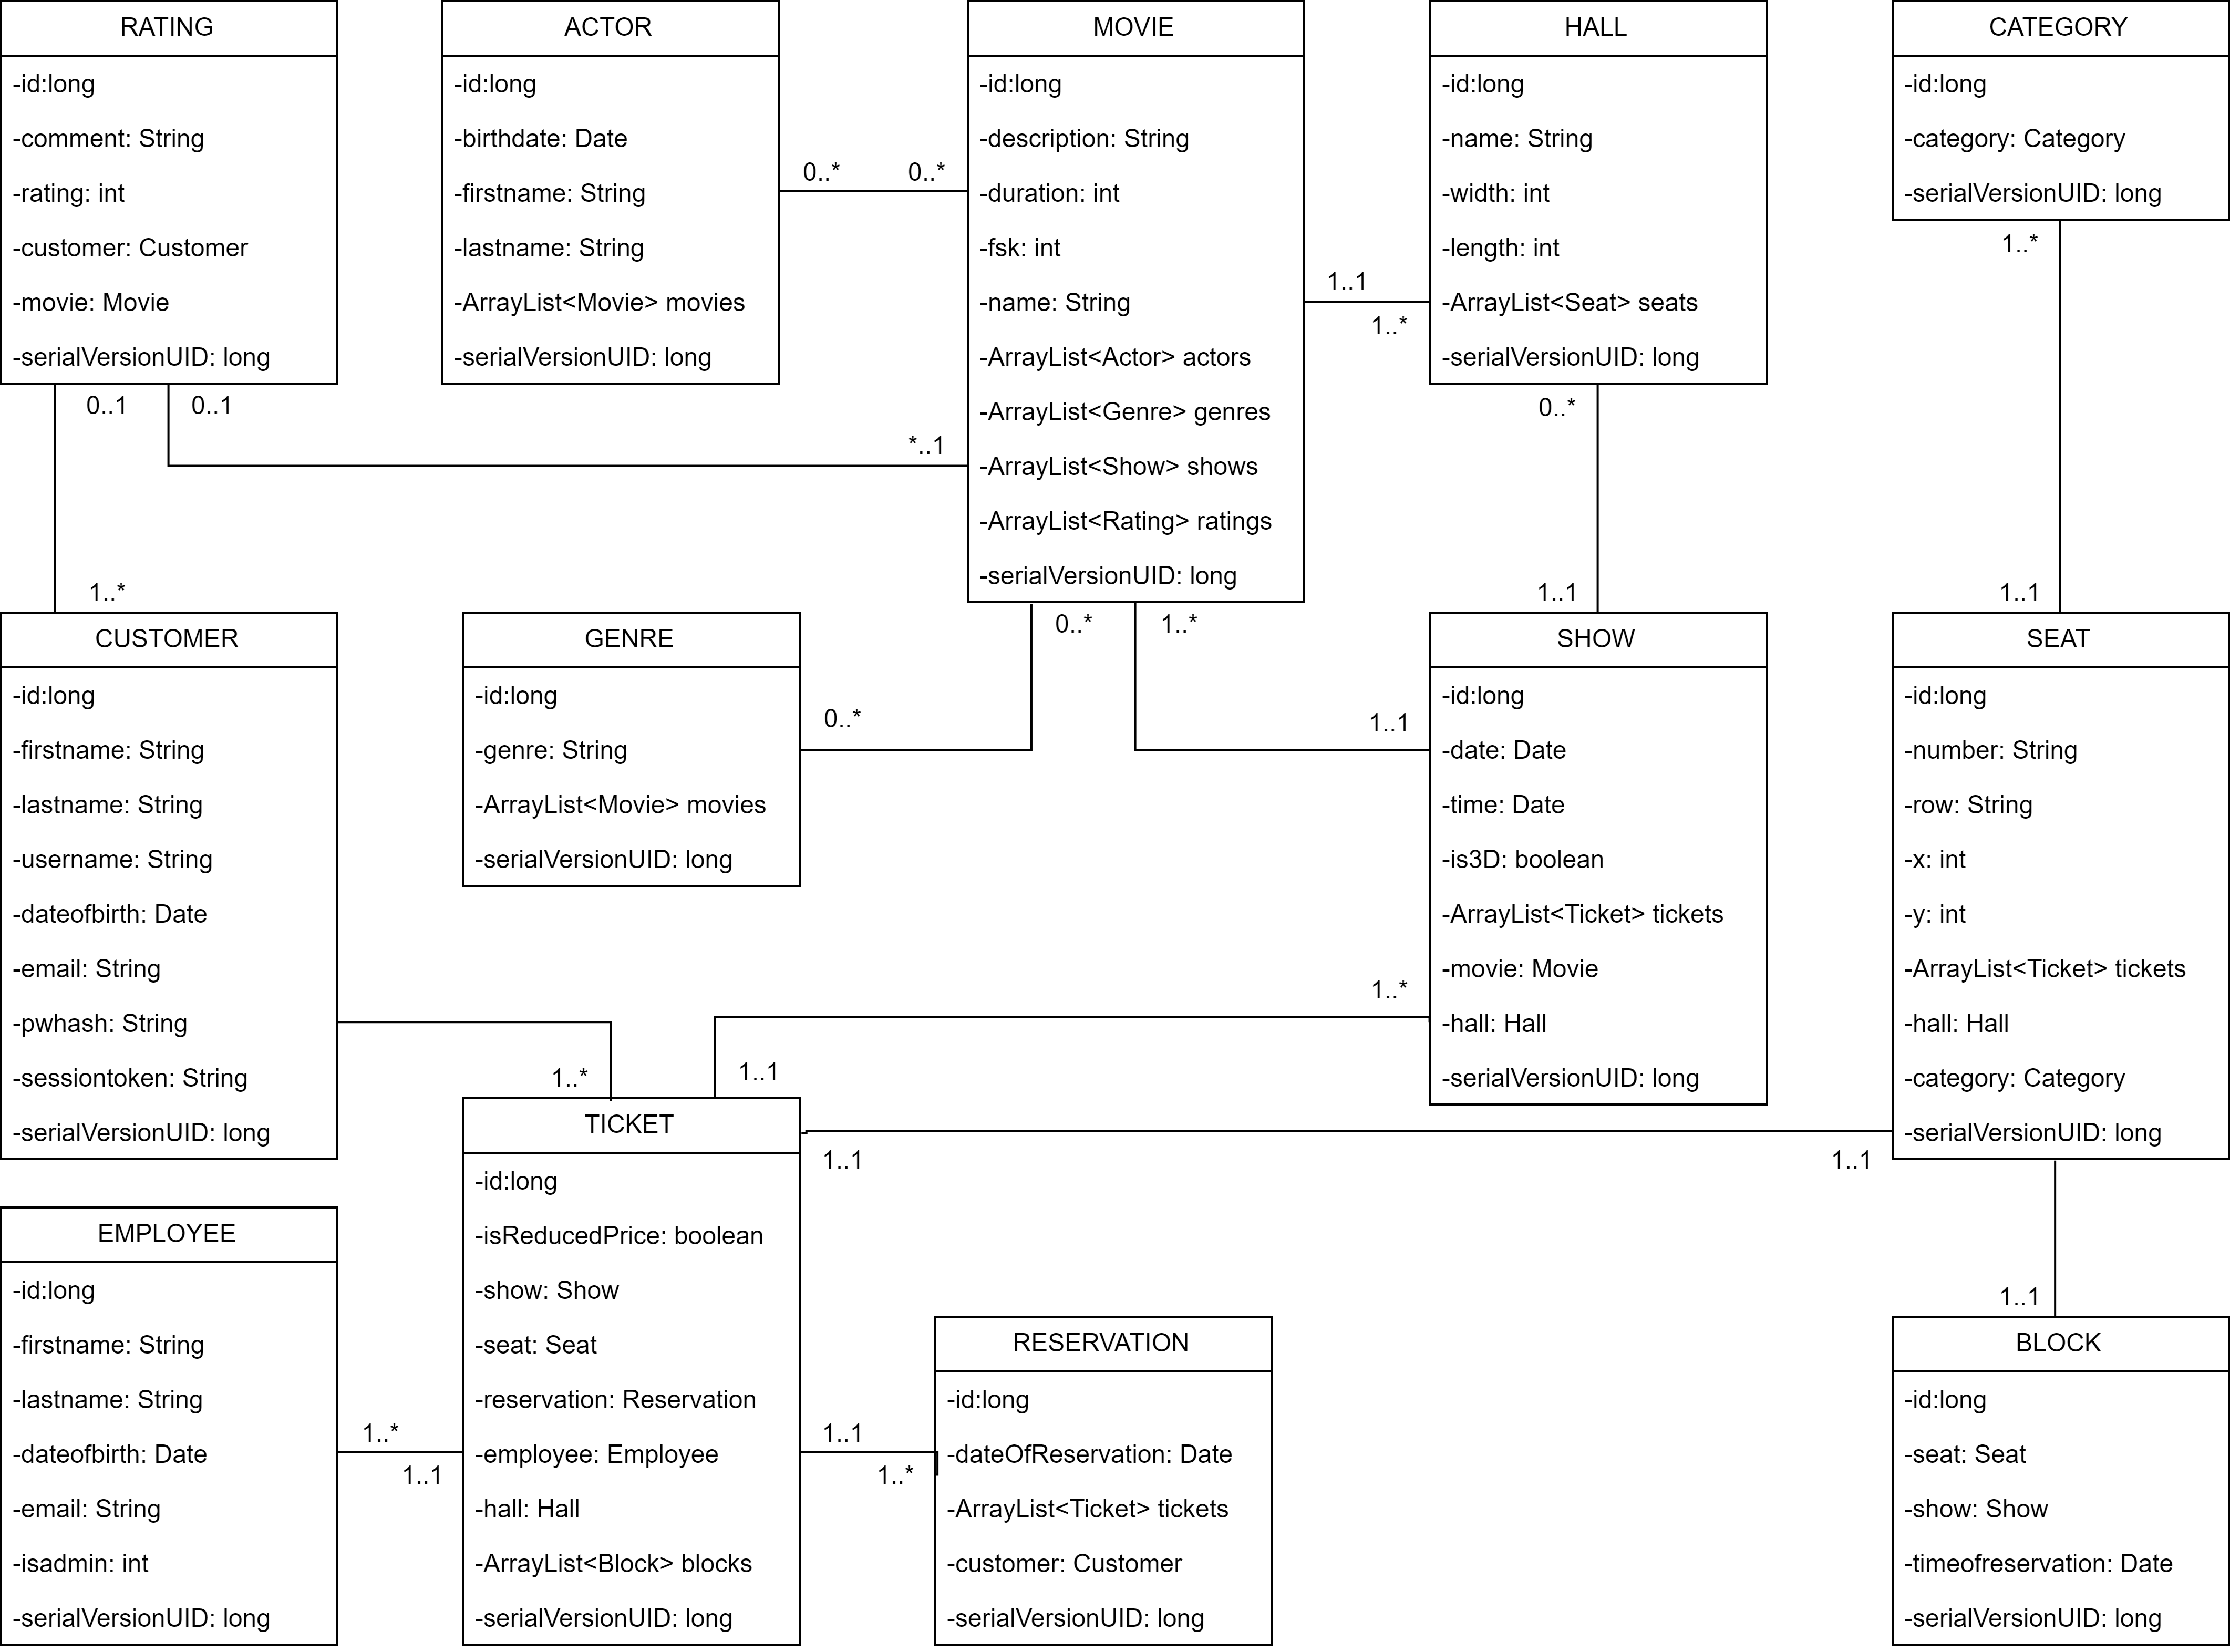
\includegraphics[keepaspectratio, width=\textwidth, height=\textheight]{img/klassendiagramm_v02}
	\captionsetup{format=hang}
	\caption{Zweiter Entwurf des Klassendiagramms}
	\small Quelle: eigene Darstellung mittels \url{https://draw.io/} 
	\label{fig:anhang_klassendiagramm02}
\end{sidewaysfigure}

\begin{sidewaysfigure}[ht]
	\centering
	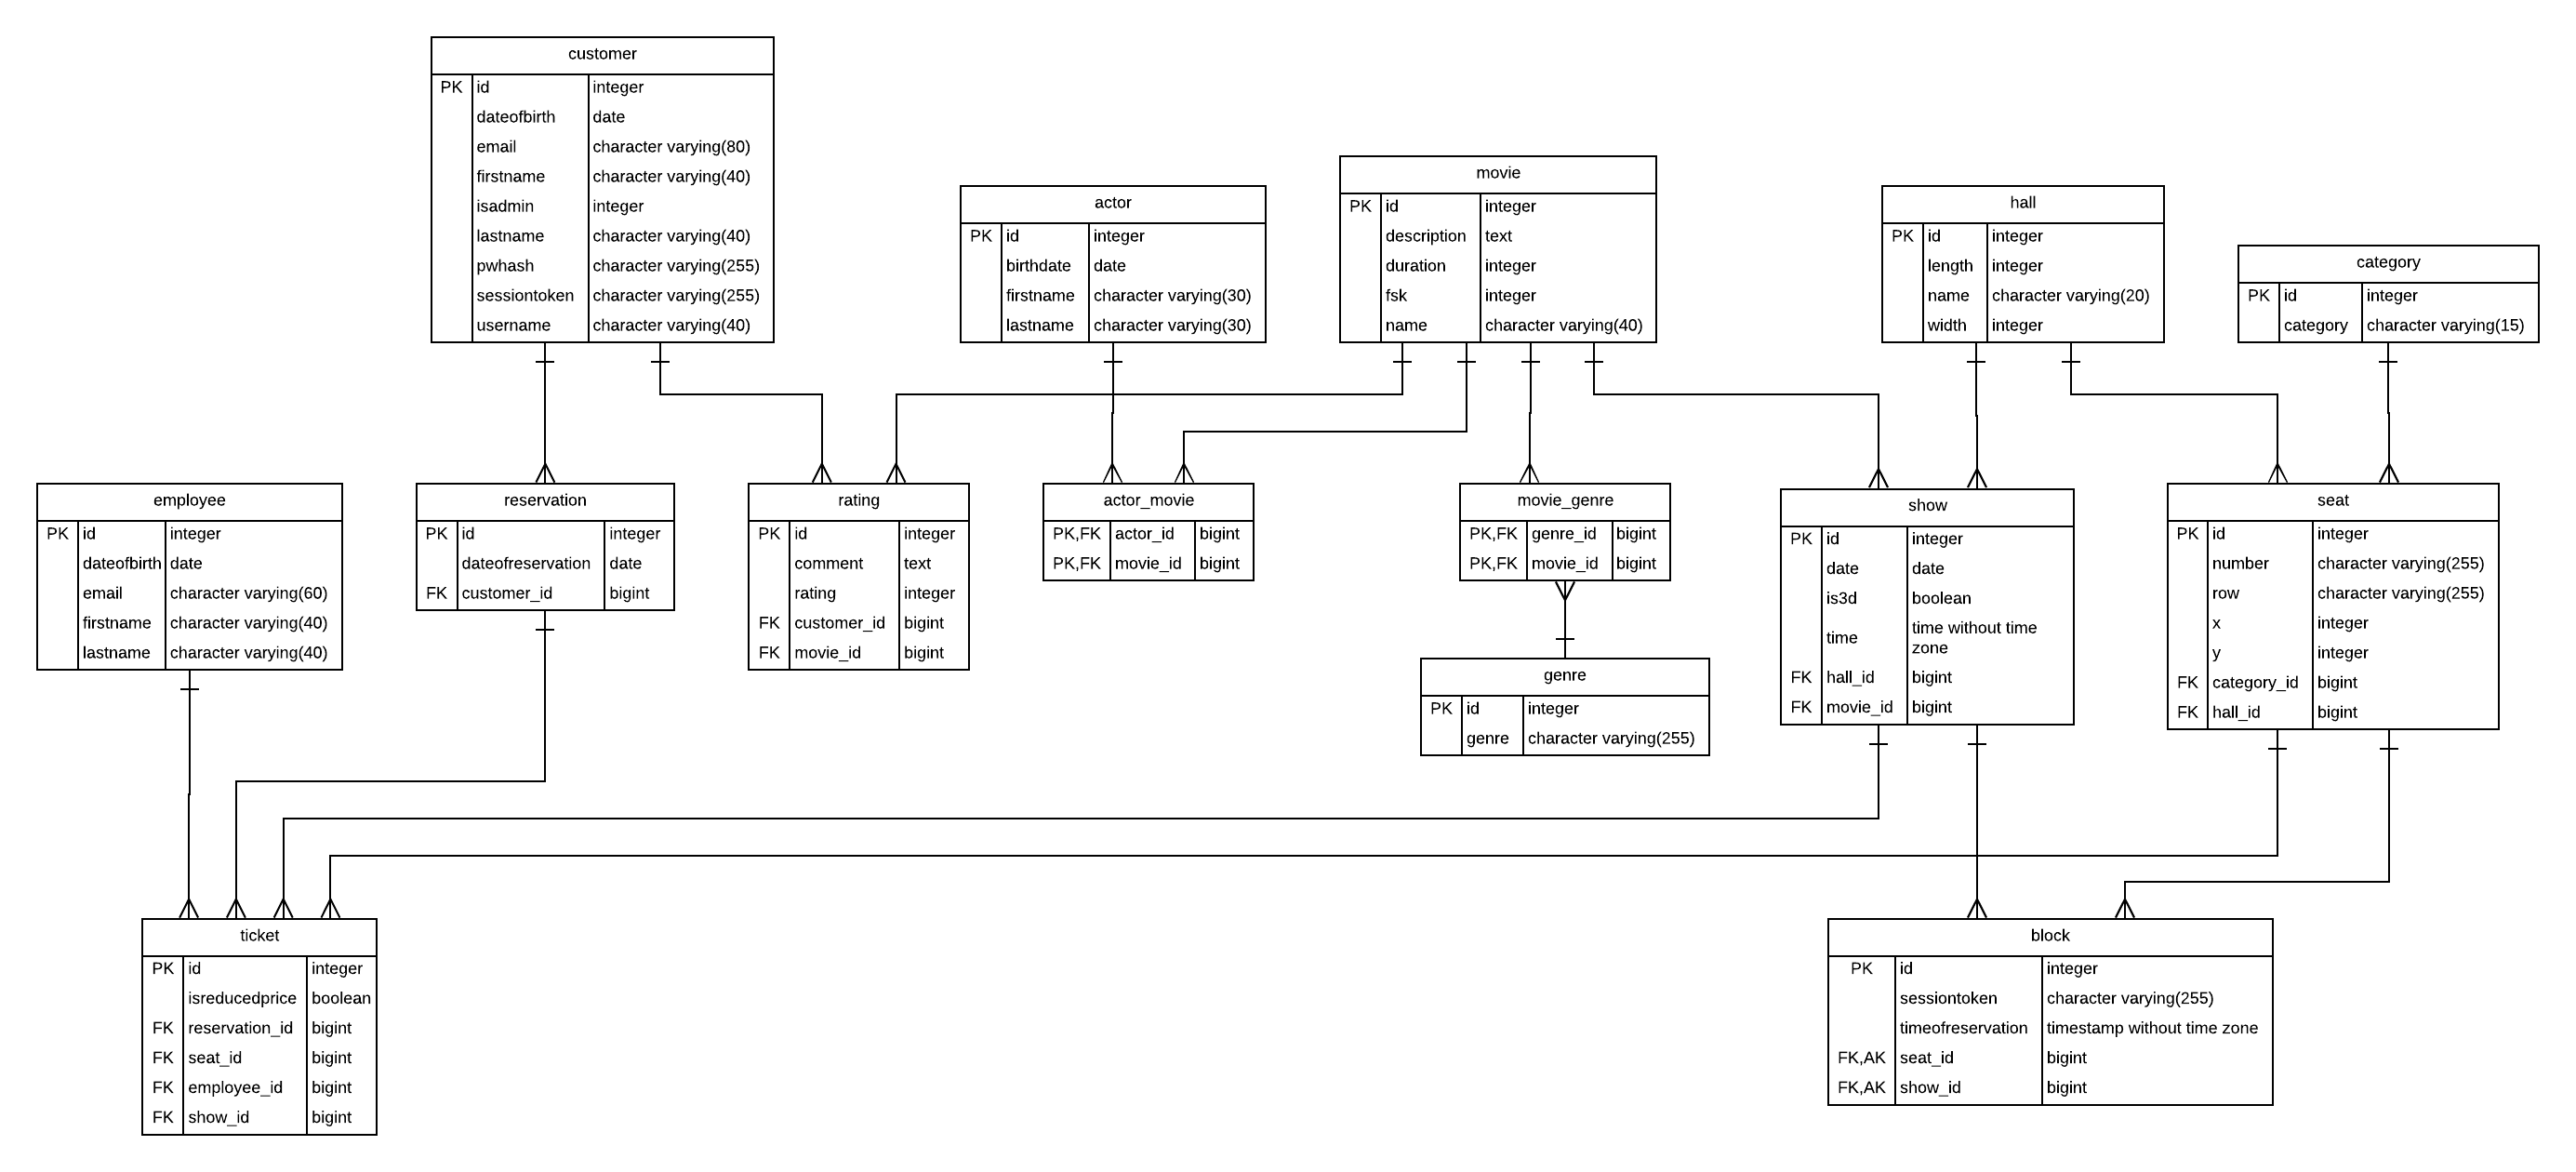
\includegraphics[keepaspectratio, width=\textwidth, height=\textheight]{img/ER-Modell}
	\captionsetup{format=hang}
	\caption{\acs{ER-Modell} der Datenbank}
	\small Quelle: eigene Darstellung mittels \url{https://www.lucidchart.com/}
	\label{fig:Anhang_ER-Modell}
\end{sidewaysfigure}

\chapter{Screenshots aus dem Front-End}
Die folgenden Screenshots sind alle von der Seite eines Filmes, wo sich weitere Details zu diesem finden.

\begin{figure}[ht]
	\centering
	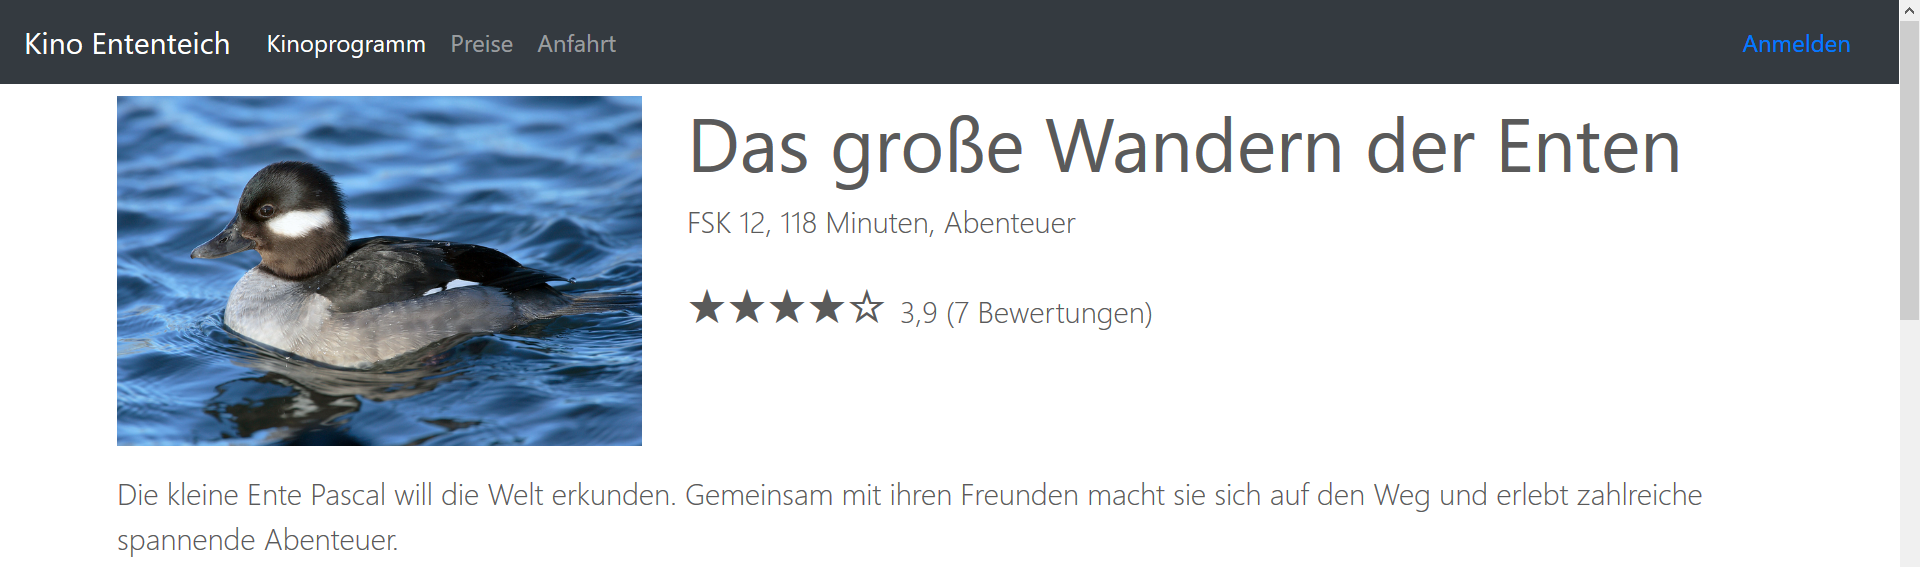
\includegraphics[width=\textwidth]{img/screenshots/film02a}
	\captionsetup{format=hang}
	\caption{Filmdetails}
	\label{fig:film02a}
\end{figure}

\begin{figure}[ht]
	\centering
	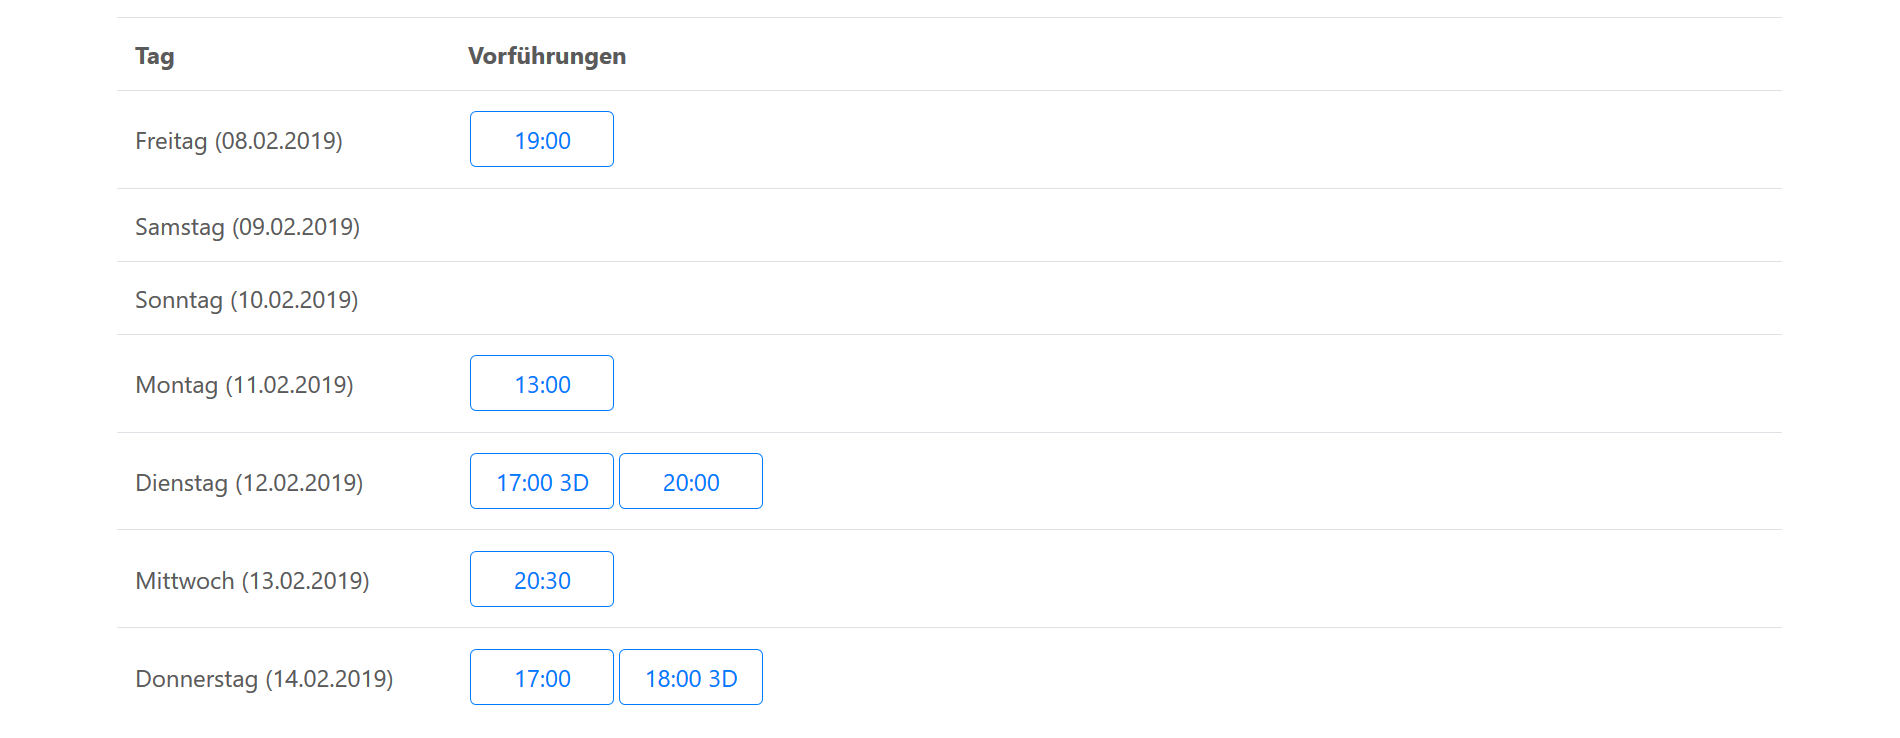
\includegraphics[width=\textwidth]{img/screenshots/film03}
	\captionsetup{format=hang}
	\caption{Liste der Vorstellungen der nächsten 7 Tage}
	\label{fig:film03}
\end{figure}

\begin{figure}[!t]
	\centering
	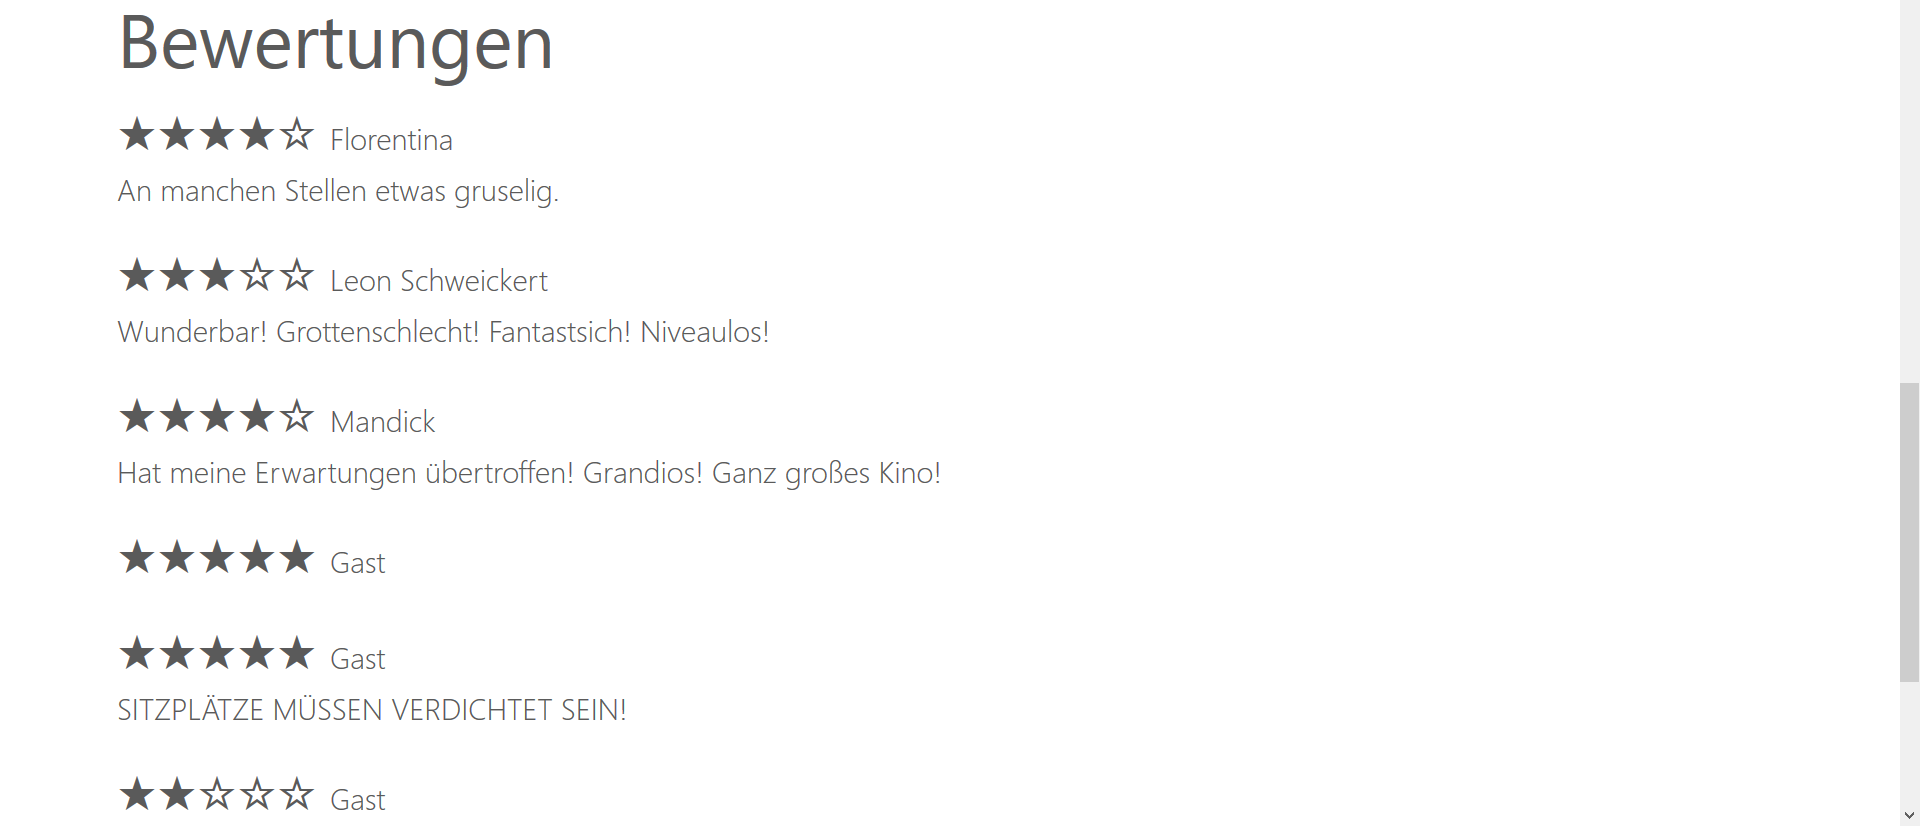
\includegraphics[width=\textwidth]{img/screenshots/film04}
	\captionsetup{format=hang}
	\caption{Bewertungen zu einem Film}
	\label{fig:film04}
\end{figure}

\chapter{Quellcode}
\begin{minipage}{\linewidth}
	\begin{lstlisting}[style=lstJava]
	public static MovieTo createMovieTo ( Movie entity, boolean withShow )
	{
	if ( null != entity )
	{
	MovieTo movieTo = new MovieTo();
	movieTo.setId(entity.getId());
	movieTo.setDescription(entity.getDescription());
	movieTo.setFsk(entity.getFsk());
	movieTo.setDuration(entity.getDuration());
	movieTo.setName(entity.getName());
	movieTo.setGenres(createGenreTos(entity.getGenres()));
	movieTo.setRatings(createRatingTos(entity.getRatings()));
	if ( withShow )
	{
	movieTo.setShows(createShowTos(entity.getShows(), false));
	} // end withSow
	movieTo.setActors(createActorTos(entity.getActors()));
	return movieTo;
	}  // end if null
	return null;
	}
	\end{lstlisting}
	\captionof{lstlisting}{Erstellen eines Movie-\acs{DTO} aus einer Movie-Entität mit Hilfe des eigen erstellten EntityToToHelper}
	\label{lst:EntityToToHelper_movie}
\end{minipage}

\begin{minipage}{\linewidth}
	\begin{lstlisting}[style=lstJava]
	public static Movie createMovieEntity ( MovieTo transferObject, boolean withShow )
	{
		if ( null != transferObject )
		{
			Movie movie = new Movie();
			movie.setId(transferObject.getId());
			movie.setActors(createActorEntities(transferObject.getActors()));
			movie.setDescription(transferObject.getDescription());
			movie.setFsk(transferObject.getFsk());
			movie.setDuration(transferObject.getDuration());
			movie.setName(transferObject.getName());
			movie.setRatings(createRatingEntities(transferObject.getRatings()));
			if ( withShow )
			{
				movie.setShows(createShowEntities(transferObject.getShows(), false));
			}
			movie.setGenres(createGenreEntities(transferObject.getGenres()));
			return movie;
		}
		return null;
	}
	\end{lstlisting}
	\captionof{lstlisting}{Erstellen einer Movie-Entität aus einem Movie-\acs{DTO} mit Hilfe des eigen erstellten ToToEntityHelper}
	\label{lst:ToToEntityHelper_movie}
\end{minipage}

\begin{minipage}{\linewidth}
	\begin{lstlisting}[style=lstJava]
	private boolean checkIfSeatsAreBookable ( List<SeatTo> seatsToProof, List<TicketTo> bookedTicketTos, List<BlockTo> blockTos, String sessiontoken )
	{
	boolean bookable = true;
	
	for ( SeatTo s : seatsToProof )
	{
	if ( bookable )
	{
	for ( TicketTo t : bookedTicketTos )
	{
	if ( s.getId() == t.getSeat().getId() )
	{
	bookable = false;
	s.setOccupied(true);
	break;
	} else
	{
	s.setOccupied(false);
	}
	} // end for ticket
	// verification for blocked elements
	for ( BlockTo b : blockTos )
	{
	if ( s.getId() == b.getSeat().getId() && !(b.getSessiontoken().equals(sessiontoken)) )
	{
	bookable = false;
	s.setBlocked(true);
	break;
	} else
	{
	s.setBlocked(false);
	}
	} // end for block
	}	// end if bookable
	}	// end for seatTo
	return bookable;
	}
	\end{lstlisting}
	\captionof{lstlisting}{Überprüfung, ob eine Reservierung möglich ist.}
	\label{lst:Angang_Prüfung_ob_Reservierung_möglich}
\end{minipage}

\begin{minipage}{\linewidth}
\begin{lstlisting}[style=lstJava]
private ReservationTo createReservationForSeats ( List<SeatTo> seatTos, ShowTo showTo )
{
	List<TicketTo> toBook = new ArrayList<>();
	ReservationTo createdReservationTo = new ReservationTo();
		
	for ( SeatTo seatTo : seatTos )
	{
		seatTo.setOccupied(true);
	
		TicketTo ticketTo = new TicketTo();
		ticketTo.setSeat(seatTo);
		ticketTo.setShow(showTo);
		ticketTo.setReservation(createdReservationTo);
		if ( seatTo.isReducedPrice() )
		{
			ticketTo.setReducedPrice(true);
		}
		toBook.add(ticketTo);
	}
	createdReservationTo.setDateOfReservation(Utils.convertDateToString(new Date()));
	createdReservationTo.setTickets(toBook);
	return createdReservationTo;
}
	\end{lstlisting}
	\captionof{lstlisting}{Erstellen eines Reservierungs-\acs{DTO}}
	\label{lst:Anhang_Erstellen_Reservierung}
\end{minipage}

\begin{minipage}{\linewidth}
  \begin{lstlisting}[style=lstJava]
  public class EntityToToHelper_Test
  {
    EntityToToHelper EtoToHelper = new EntityToToHelper();

    @Before
    public void initialize ( )
    {
      EmployeeTo testEmployeeTo = new EmployeeTo();
      testEmployeeTo.setId(1);
      testEmployeeTo.setDateofbirth(testDateString);
      testEmployeeTo.setEmail("mail");
      testEmployeeTo.setFirstname("firstname");
      testEmployeeTo.setLastname("lastname");

      Employee testEmployeeEntity = new Employee();
      testEmployeeEntity.setId(1);
      testEmployeeEntity.setDateofbirth(testDateDate);
      testEmployeeEntity.setEmail("mail");
      testEmployeeEntity.setFirstname("firstname");
      testEmployeeEntity.setLastname("lastname");
    }

    @Test
    public void testCreateEmployeeTo ( )
    {
      assertEquals(null, EtoToHelper.createEmployeeTo(null));

      EmployeeTo compareEmployeeTo = EtoToHelper.createEmployeeTo(testEmployeeEntity);

      assertThat(testEmployeeTo.getId(), equalTo(compareEmployeeTo.getId()));
      assertThat(testEmployeeTo.getDateofbirth(), equalTo(compareEmployeeTo.getDateofbirth()));
      assertThat(testEmployeeTo.getEmail(), equalTo(compareEmployeeTo.getEmail()));
      assertThat(testEmployeeTo.getFirstname(), equalTo(compareEmployeeTo.getFirstname()));
      assertThat(testEmployeeTo.getLastname(), equalTo(compareEmployeeTo.getLastname()));
    }
  }

	\end{lstlisting}
	\captionof{lstlisting}{Ausschnitt der Test-Klasse der EntityToToHelper-Klasse}
  \label{src:entitytotohelpertest}
\end{minipage}